\documentclass[aspectratio=169]{beamer}

\usepackage[utf8]{inputenc}
\usepackage[english]{babel}
\usepackage{booktabs}
\usepackage{array}
\usepackage{framed}
\usepackage{graphicx}
\usepackage{tikz}
\usetikzlibrary{arrows.meta,positioning,fit,calc,shapes.geometric}
\usepackage{empheq}
\usepackage{tcolorbox}
\tcbuselibrary{skins,theorems}
\usepackage{listings}
\usepackage{xcolor}

\newtcbox{\mymath}[1][]{%
    nobeforeafter, math upper, tcbox raise base,
    enhanced, colframe=blue!30!black,
    colback=blue!30, boxrule=1pt,
    #1}

\graphicspath{{logo/}{../logo/}{figures/}{../figures/}}

\definecolor{ForestGreen}{RGB}{22,100,70}
\definecolor{SoftGreen}{RGB}{229,244,235}
\definecolor{SoftBlue}{RGB}{226,239,255}
\definecolor{SoftOrange}{RGB}{255,241,220}
\definecolor{SoftPurple}{RGB}{239,231,255}
\definecolor{CodeGray}{RGB}{247,247,247}

\newcolumntype{L}[1]{>{\raggedright\arraybackslash}p{#1}}

\mode<presentation>{
  \usetheme{Ilmenau}
  \usecolortheme{spruce}
  \usefonttheme{professionalfonts}
  \setbeamertemplate{navigation symbols}{}
  \setbeamertemplate{headline}{}
  \setbeamertemplate{caption}[numbered]
  \setbeamercolor{institute in head/foot}{fg=ForestGreen}
  \setbeamercolor{metric box}{bg=ForestGreen,fg=white}
}

\lstdefinestyle{pythonstyle}{
  language=Python,
  backgroundcolor=\color{CodeGray},
  basicstyle=\ttfamily\scriptsize,
  keywordstyle=\color{blue!70!black}\bfseries,
  stringstyle=\color{ForestGreen!90!black},
  commentstyle=\color{gray!80!black}\itshape,
  numbers=left,
  numberstyle=\tiny\color{gray},
  stepnumber=1,
  numbersep=7pt,
  showstringspaces=false,
  frame=single,
  rulecolor=\color{ForestGreen!50},
  breaklines=true,
  tabsize=4,
  columns=fullflexible
}
\lstset{style=pythonstyle}

\tikzset{
  concept/.style={draw=ForestGreen, rounded corners, fill=SoftGreen,
    very thick, minimum height=1.15cm, text width=3.6cm, align=center},
  application/.style={draw=blue!60!black, rounded corners, fill=SoftBlue,
    thick, minimum height=0.95cm, text width=3.8cm, align=center},
  stage/.style={draw=ForestGreen, rounded corners, fill=SoftGreen,
    thick, minimum height=1.15cm, text width=2.05cm, align=center,
    font=\small},
  smallstage/.style={draw=ForestGreen, rounded corners, fill=SoftGreen,
    thick, minimum height=0.9cm, text width=1.8cm, align=center,
    font=\scriptsize},
  typebox/.style={draw=blue!60!black, rounded corners, fill=SoftBlue,
    thick, minimum height=1.0cm, text width=2.4cm, align=center},
  adtbox/.style={draw=purple!70!black, rounded corners, fill=SoftPurple,
    thick, minimum height=1.0cm, text width=2.8cm, align=center},
  arrow/.style={-Latex, very thick, ForestGreen}
}


% -------------------------------------------------------------
% Logo fallbacks and quiz helper
% -------------------------------------------------------------
\newcommand{\TitleLogo}{%
  \IfFileExists{logo/logo_slide.png}{\includegraphics[width=0.27\textwidth]{logo/logo_slide.png}}{%
  \IfFileExists{../logo/logo_slide.png}{\includegraphics[width=0.27\textwidth]{../logo/logo_slide.png}}{%
  \IfFileExists{logo_slide.png}{\TitleLogo}{%
  \fcolorbox{ForestGreen}{ForestGreen}{\parbox[c][0.85cm][c]{0.27\textwidth}{\centering\color{white}\bfseries NEU -- DS\&AI}}}}}%
}
\newcommand{\FooterLogo}{%
  \IfFileExists{logo/logo_fda.png}{\includegraphics[width=0.8cm]{logo/logo_fda.png}}{%
  \IfFileExists{../logo/logo_fda.png}{\includegraphics[width=0.8cm]{../logo/logo_fda.png}}{%
  \IfFileExists{logo_fda.png}{\includegraphics[width=0.8cm]{logo_fda.png}}{%
  \fcolorbox{ForestGreen}{ForestGreen}{\parbox[c][0.45cm][c]{0.8cm}{\centering\color{white}\scriptsize FDA}}}}}%
}
\newcommand{\quizblock}[1]{%
  \begin{alertblock}{Quiz / Quick check}
    #1
  \end{alertblock}
}

\title[TOKT11105 - Lecture 1]{Data Structures and Algorithms in Python\\Lecture 1 -- Part II: Programming Foundations and ADTs}
\author{Faculty of Data Science and Artificial Intelligence}
\institute{College of Technology - National Economics University}
\date{}

\AtBeginSection[]{
  \begin{frame}[plain]
    \begin{center}
      \vfill
      {\color{ForestGreen}\large\bfseries SECTION \insertsectionnumber}

      \vspace{0.8em}
      {\color{ForestGreen}\rule{0.68\textwidth}{1.2pt}}

      \vspace{1.1em}
      {\usebeamerfont{section title}\color{ForestGreen}\Huge\bfseries
        \insertsectionhead}

      \vspace{1.1em}
      {\color{ForestGreen}\rule{0.68\textwidth}{1.2pt}}
      \vfill
    \end{center}
  \end{frame}
}

\begin{document}

% =============================================================
% TITLE
% =============================================================
\begin{frame}[plain]
  \setbeamercolor{block body example}{bg=ForestGreen,fg=white}
  \begin{center}
    \begin{beamercolorbox}[wd=\textwidth,sep=1pt,center,rounded=true,shadow=true]{block body example}
      \TitleLogo
    \end{beamercolorbox}
  \end{center}
  \vspace{-0.25em}
  \titlepage
\end{frame}

\logo{\FooterLogo}
\setbeamertemplate{footline}{%
  \begin{beamercolorbox}[colsep=1.5pt]{upper separation line foot}
  \end{beamercolorbox}
  \begin{beamercolorbox}[ht=2.5ex,dp=1.125ex,leftskip=.3cm,rightskip=.3cm]{author in head/foot}%
    \leavevmode{\usebeamerfont{author in head/foot}\insertshortauthor}%
    \hfill%
    {\usebeamerfont{institute in head/foot}\usebeamercolor[fg]{institute in head/foot}\insertshortinstitute}%
    \hfill%
    {\usebeamerfont{institute in head/foot}\usebeamercolor[fg]{institute in head/foot}\insertframenumber{} / \inserttotalframenumber}%
  \end{beamercolorbox}%
  \begin{beamercolorbox}[colsep=1.5pt]{lower separation line foot}
  \end{beamercolorbox}%
}

% =============================================================
% OPENING
% =============================================================
\begin{frame}{Where we are in Lecture 1}
  \begin{center}
    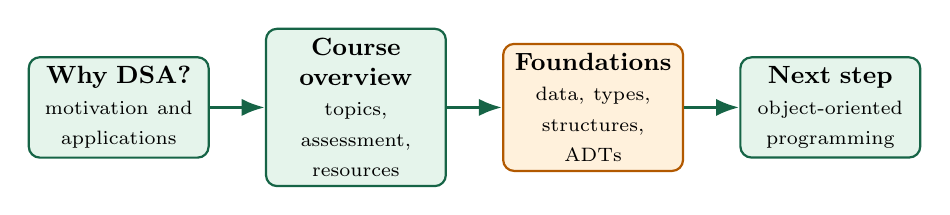
\begin{tikzpicture}[node distance=0.7cm]
      \node[stage] (why) {\textbf{Why DSA?}\\\scriptsize motivation and applications};
      \node[stage, right=of why] (course) {\textbf{Course overview}\\\scriptsize topics, assessment, resources};
      \node[stage, right=of course, fill=SoftOrange, draw=orange!70!black] (foundation) {\textbf{Foundations}\\\scriptsize data, types, structures, ADTs};
      \node[stage, right=of foundation] (next) {\textbf{Next step}\\\scriptsize object-oriented programming};
      \draw[arrow] (why) -- (course);
      \draw[arrow] (course) -- (foundation);
      \draw[arrow] (foundation) -- (next);
    \end{tikzpicture}
  \end{center}

  \vspace{0.8em}
  \begin{alertblock}{Main question for this half}
    Before designing efficient algorithms, how should we represent, organize,
    and interact with data?
  \end{alertblock}
\end{frame}

\begin{frame}{Learning outcomes}
  By the end of this part, you should be able to:
  \begin{enumerate}
    \item explain how Python represents data as values accessed through variable names;
    \item distinguish primitive/basic values from collection types;
    \item define, classify, and choose a data structure from the operations a problem requires;
    \item explain an Abstract Data Type (ADT) as a public contract;
    \item distinguish an ADT from its concrete implementation.
  \end{enumerate}

  \vspace{0.6em}
  \begin{empheq}[box=\tcbhighmath]{equation*}
    \text{Data $\rightarrow$ Values $\rightarrow$ Types $\rightarrow$ Organization $\rightarrow$ Operations}
  \end{empheq}
\end{frame}

% =============================================================
\section{Data}
% =============================================================

\begin{frame}[fragile]{Data in a Python program}
  \begin{columns}[T]
    \begin{column}{0.46\textwidth}
      \begin{block}{What is data?}
        Data are facts or observations that a program stores, processes, and
        produces.
      \end{block}

      \begin{exampleblock}{How Python represents data}
        Python represents data as \textbf{values}. A variable gives a value a
        meaningful name so the program can use it.
      \end{exampleblock}
    \end{column}
    \begin{column}{0.50\textwidth}
\begin{lstlisting}
student_name = "An"
student_id = 2026001
gpa = 3.42
is_active = True
\end{lstlisting}

      \begin{alertblock}{Examples of represented data}
        Text, identifiers, measurements, and logical conditions become Python
        values that a program can manipulate.
      \end{alertblock}
    \end{column}
  \end{columns}
\end{frame}

\begin{frame}[fragile]{Working with data through variables}
  \begin{columns}[T]
    \begin{column}{0.47\textwidth}
\begin{lstlisting}
balance = 1000
deposit = 250

balance = balance + deposit
print(balance)       # 1250
\end{lstlisting}
    \end{column}
    \begin{column}{0.49\textwidth}
      \begin{block}{Names make data usable}
        \texttt{balance} and \texttt{deposit} describe the meaning of their
        values and allow those values to be used in an expression.
      \end{block}

      \begin{exampleblock}{Assignment updates program state}
        The new result is assigned to \texttt{balance}. The program can then
        read the updated value later.
      \end{exampleblock}
    \end{column}
  \end{columns}
\end{frame}

\begin{frame}[fragile]{The same mutable data can have two names}
  \begin{center}
    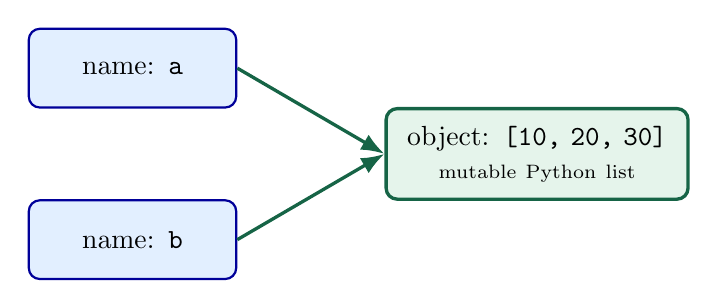
\begin{tikzpicture}[node distance=2.0cm]
      \node[typebox] (a) {name: \texttt{a}};
      \node[typebox, below=1.15cm of a] (b) {name: \texttt{b}};
      \node[concept, right=3.2cm of $(a)!0.5!(b)$] (list) {object: \texttt{[10, 20, 30]}\\\scriptsize mutable Python list};
      \draw[arrow] (a.east) -- (list.west);
      \draw[arrow] (b.east) -- (list.west);
    \end{tikzpicture}
  \end{center}

  \vspace{0.4em}
\begin{lstlisting}
a = [10, 20, 30]
b = a
b.append(40)
print(a)        # [10, 20, 30, 40]
\end{lstlisting}

  \begin{alertblock}{Why does \texttt{a} change?}
    Both names refer to the same mutable object.
  \end{alertblock}
\end{frame}

\begin{frame}[fragile]{Quick check: shared data or copied data?}
  \small
  \begin{columns}[T]
    \begin{column}{0.48\textwidth}
      \begin{block}{Predict both outputs}
\begin{lstlisting}
scores = [8, 7]
shared = scores
copied = scores.copy()
shared.append(9)
print(scores)
print(copied)
\end{lstlisting}
      \end{block}
    \end{column}
    \begin{column}{0.48\textwidth}
      \quizblock{
      Without running the code, decide which statement is correct.
      \begin{enumerate}
        \item Both printed lists are the same.
        \item Only \texttt{scores} changes.
        \item Only \texttt{copied} changes.
        \item Neither list changes.
      \end{enumerate}}
      \begin{exampleblock}{Discussion prompt}
        Explain the difference between assigning a new name to a mutable object
        and creating an independent copy.
      \end{exampleblock}
    \end{column}
  \end{columns}
\end{frame}


\begin{frame}{Quiz: data, value, variable, object}
\small
\quizblock{
Classify each statement as referring mainly to a \textbf{variable name}, a
\textbf{value}, a \textbf{type}, or an \textbf{object reference}.
}
\vspace{0.35em}
\begin{enumerate}
  \item In \texttt{gpa = 3.42}, \texttt{gpa} is the item used by the program to access data.
  \item \texttt{3.42} is the stored numeric value.
  \item \texttt{float} describes the kind of value and valid operations.
  \item Two names may refer to the same mutable list.
\end{enumerate}
\vspace{0.35em}
\begin{alertblock}{Follow-up}
Why is this distinction important when a program modifies a list or dictionary?
\end{alertblock}
\end{frame}

% =============================================================
\section{Data Types}
% =============================================================

\begin{frame}{What is a data type?}
  \begin{columns}[T]
    \begin{column}{0.46\textwidth}
      \begin{block}{Definition}
        A data type identifies a set of possible values and the operations that
        are meaningful for those values.
      \end{block}

      \begin{exampleblock}{Why types matter}
        Types help the language interpret stored bits and decide which
        operations are valid.
      \end{exampleblock}
    \end{column}
    \begin{column}{0.50\textwidth}
      \begin{center}
        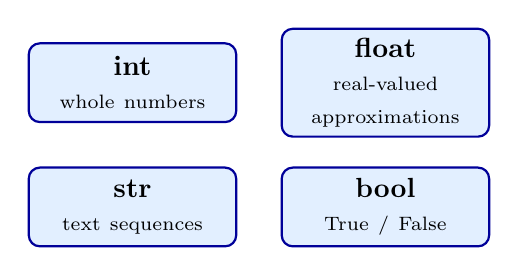
\begin{tikzpicture}[node distance=0.55cm]
          \node[typebox] (int) {\textbf{int}\\\scriptsize whole numbers};
          \node[typebox, right=of int] (float) {\textbf{float}\\\scriptsize real-valued approximations};
          \node[typebox, below=of int] (str) {\textbf{str}\\\scriptsize text sequences};
          \node[typebox, right=of str] (bool) {\textbf{bool}\\\scriptsize True / False};
        \end{tikzpicture}
      \end{center}
    \end{column}
  \end{columns}
\end{frame}

\begin{frame}{Primitive (basic) data types in Python}
  \begin{center}
    \setlength{\tabcolsep}{4pt}
    \begin{tabular}{L{0.16\textwidth}L{0.23\textwidth}L{0.27\textwidth}L{0.22\textwidth}}
      \toprule
      \textbf{Type} & \textbf{Example} & \textbf{Typical meaning} & \textbf{Example operation} \\
      \midrule
      \texttt{int} & \texttt{2026001} & identifier, count & \texttt{+}, \texttt{-}, \texttt{//} \\
      \addlinespace
      \texttt{float} & \texttt{3.42} & measurement, score & \texttt{+}, \texttt{*}, \texttt{/} \\
      \addlinespace
      \texttt{str} & \texttt{"Nguyen An"} & text & concatenation, indexing \\
      \addlinespace
      \texttt{bool} & \texttt{True} & logical condition & \texttt{and}, \texttt{or}, \texttt{not} \\
      \bottomrule
    \end{tabular}
  \end{center}

  \vspace{0.15em}
  \begin{alertblock}{Course convention}
    We use \emph{primitive/basic} for these fundamental built-in values. Python
    treats every value as an object and has no separate \texttt{char} type;
    \texttt{"A"} is a string of length one.
  \end{alertblock}
\end{frame}

\begin{frame}[fragile]{The same operator may behave differently}
  \footnotesize
  \begin{columns}[T]
    \begin{column}{0.48\textwidth}
\begin{lstlisting}[basicstyle=\ttfamily\scriptsize]
print(2 + 3)              # 5
print(2.0 + 3.0)          # 5.0
print("data" + "science")  # datascience
print([1, 2] + [3, 4])    # [1, 2, 3, 4]

print(2 + "3")            # TypeError
\end{lstlisting}

      \begin{alertblock}{No automatic conversion}
        Python does not silently convert \texttt{"3"} to the integer
        \texttt{3}. Use \texttt{2 + int("3")} when conversion is intended.
      \end{alertblock}
    \end{column}
    \begin{column}{0.48\textwidth}
      \begin{block}{Type-directed meaning of \texttt{+}}
        \begin{itemize}
          \item \texttt{int + int} $\rightarrow$ integer addition;
          \item \texttt{float + float} $\rightarrow$ floating-point addition;
          \item \texttt{str + str} $\rightarrow$ string concatenation;
          \item \texttt{list + list} $\rightarrow$ list concatenation.
        \end{itemize}
      \end{block}

      \begin{exampleblock}{Runtime decision}
        Python examines the operand types and selects the operation supported
        by those types. An unsupported combination raises \texttt{TypeError}.
      \end{exampleblock}
    \end{column}
  \end{columns}

  \vspace{0.2em}
  \begin{alertblock}{Key lesson}
    A data type determines which operators are valid, what they mean, and the
    type of result they produce.
  \end{alertblock}
\end{frame}

\begin{frame}{Non-primitive built-in collection types}
  \small
  \begin{columns}[T]
    \begin{column}{0.48\textwidth}
      \begin{block}{Sequences}
        \begin{itemize}
          \item \texttt{list}: ordered and mutable
          \item \texttt{tuple}: ordered and immutable
        \end{itemize}
      \end{block}
      \begin{exampleblock}{Examples}
        \texttt{[500000, -200000, 1000000]}\\[0.3em]
        \texttt{("Hanoi", 21.5)}
      \end{exampleblock}
    \end{column}
    \begin{column}{0.48\textwidth}
      \begin{block}{Mappings and sets}
        \begin{itemize}
          \item \texttt{dict}: key--value mapping
          \item \texttt{set}: unique values
        \end{itemize}
      \end{block}
      \begin{exampleblock}{Examples}
        \texttt{\char123"id": 105, "balance": 2.5e7\char125}\\[0.3em]
        \texttt{\char123"ATM", "Mobile Banking"\char125}
      \end{exampleblock}
    \end{column}
  \end{columns}
\end{frame}

\begin{frame}{Primitive versus non-primitive data types}
  \small
  \begin{center}
    \setlength{\tabcolsep}{4pt}
    \begin{tabular}{L{0.18\textwidth}L{0.36\textwidth}L{0.36\textwidth}}
      \toprule
      \textbf{Aspect} & \textbf{Primitive / basic} & \textbf{Non-primitive / composite} \\
      \midrule
      Main role & Represent a fundamental value directly & Organize multiple values or fields \\
      \addlinespace
      Python examples & \texttt{int}, \texttt{float}, \texttt{bool}, \texttt{str} &
        \texttt{list}, \texttt{tuple}, \texttt{dict}, \texttt{set}, user-defined classes \\
      \addlinespace
      Typical operations & Arithmetic, comparison, logic, and text operations &
        Indexing, iteration, membership, key lookup, and object methods \\
      \addlinespace
      Mutability & The examples above are immutable & May be mutable or immutable \\
      \bottomrule
    \end{tabular}
  \end{center}


\end{frame}

\begin{frame}{Choosing a collection by behavior}
  \begin{center}
    \setlength{\tabcolsep}{5pt}
    \begin{tabular}{L{0.29\textwidth}L{0.16\textwidth}L{0.16\textwidth}L{0.20\textwidth}}
      \toprule
      \textbf{Requirement} & \textbf{Order?} & \textbf{Duplicates?} & \textbf{Candidate} \\
      \midrule
      Daily transaction sequence & Yes & Yes & \texttt{list} \\
      \addlinespace
      Geographic coordinate & Yes & Yes & \texttt{tuple} \\
      \addlinespace
      Customer record by field name & By key & Keys unique & \texttt{dict} \\
      \addlinespace
      Unique registered services & No fixed order & No & \texttt{set} \\
      \bottomrule
    \end{tabular}
  \end{center}

  \vspace{0.5em}
  \centering
  \Large Choose a type because of the behavior the problem requires.
\end{frame}


\begin{frame}{Quiz: choosing an appropriate Python type}
\small
\quizblock{For each requirement, choose one candidate type: \texttt{int}, \texttt{float}, \texttt{str}, \texttt{bool}, \texttt{list}, \texttt{tuple}, \texttt{dict}, or \texttt{set}.}
\vspace{0.3em}
\begin{enumerate}
  \item Store whether a student is currently active.
  \item Store a student's full name.
  \item Store the ordered sequence of daily sales values.
  \item Store a fixed coordinate such as latitude and longitude.
  \item Store a customer record indexed by field names such as \texttt{name} and \texttt{balance}.
  \item Store unique course codes without duplicates.
\end{enumerate}
\end{frame}

\begin{frame}[fragile]{Quiz: operator behavior depends on type}
\small
\begin{columns}[T]
\begin{column}{0.52\textwidth}
\begin{lstlisting}[basicstyle=\ttfamily\scriptsize]
print(10 + 5)
print("10" + "5")
print([10] + [5])
print(10 + "5")
\end{lstlisting}
\end{column}
\begin{column}{0.44\textwidth}
\quizblock{
For each line, predict whether Python performs arithmetic addition,
concatenation, list concatenation, or raises an error.
}
\begin{exampleblock}{Explain}
Which operand types does Python see in each expression?
\end{exampleblock}
\end{column}
\end{columns}
\end{frame}

% =============================================================
\section{Data Structures}
% =============================================================

\begin{frame}{From data types to data structures}
  \begin{columns}[T]
    \begin{column}{0.47\textwidth}
      \begin{block}{Data type asks}
        What kind of value is this, and which operations are valid?
      \end{block}

      \begin{exampleblock}{Data structure asks}
        How should many values be organized so that important operations can
        be performed efficiently?
      \end{exampleblock}
    \end{column}
    \begin{column}{0.49\textwidth}
      \begin{center}
        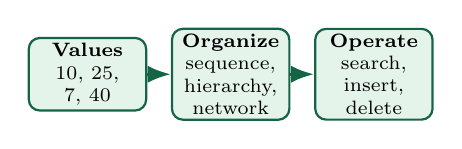
\begin{tikzpicture}[node distance=0.30cm]
          \node[smallstage,text width=1.35cm,inner sep=2pt] (values) {\textbf{Values}\\10, 25, 7, 40};
          \node[smallstage,text width=1.35cm,inner sep=2pt, right=of values] (organize) {\textbf{Organize}\\sequence, hierarchy, network};
          \node[smallstage,text width=1.35cm,inner sep=2pt, right=of organize] (operate) {\textbf{Operate}\\search, insert, delete};
          \draw[arrow] (values) -- (organize);
          \draw[arrow] (organize) -- (operate);
        \end{tikzpicture}
      \end{center}

      \vspace{0.5em}
      \begin{alertblock}{Definition}
        A data structure is a particular way of storing and organizing data so
        it can be used effectively.
      \end{alertblock}
    \end{column}
  \end{columns}
\end{frame}

\begin{frame}{Linear and non-linear data structures}
  \begin{columns}[T]
    \begin{column}{0.48\textwidth}
      \begin{block}{Linear structures}
        Elements are logically arranged in a sequence.
      \end{block}
      \begin{center}
        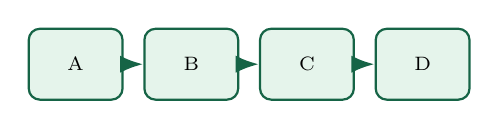
\begin{tikzpicture}[node distance=0.25cm]
          \node[smallstage,text width=1.05cm,inner sep=2pt] (a) {A};
          \node[smallstage,text width=1.05cm,inner sep=2pt, right=of a] (b) {B};
          \node[smallstage,text width=1.05cm,inner sep=2pt, right=of b] (c) {C};
          \node[smallstage,text width=1.05cm,inner sep=2pt, right=of c] (d) {D};
          \draw[arrow] (a) -- (b);
          \draw[arrow] (b) -- (c);
          \draw[arrow] (c) -- (d);
        \end{tikzpicture}
      \end{center}
      \centering Python lists, arrays, and linked lists
    \end{column}
    \begin{column}{0.48\textwidth}
      \begin{exampleblock}{Non-linear structures}
        Elements form hierarchical or network relationships.
      \end{exampleblock}
      \begin{center}
        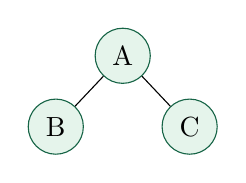
\begin{tikzpicture}[level distance=0.9cm,
          every node/.style={draw=ForestGreen,fill=SoftGreen,circle,minimum size=0.7cm},
          level 1/.style={sibling distance=1.7cm}]
          \node {A}
            child {node {B}}
            child {node {C}};
        \end{tikzpicture}
      \end{center}
      \centering Trees and graphs
    \end{column}
  \end{columns}
\end{frame}
\begin{frame}{Example: choose a structure for the workload}
  \footnotesize
  \begin{block}{Scenario and required operations}
    Store the unique student IDs allowed to enter a laboratory.
    \texttt{contains(id)} is very frequent; \texttt{add(id)} and
    \texttt{remove(id)} are occasional; order and index positions are not needed.
  \end{block}

  \begin{center}
    \setlength{\tabcolsep}{4pt}
    \renewcommand{\arraystretch}{1.03}
    \begin{tabular}{L{0.13\textwidth}L{0.20\textwidth}L{0.22\textwidth}L{0.34\textwidth}}
      \toprule
      \textbf{Candidate} & \textbf{Membership test} & \textbf{Add / remove} & \textbf{Other behavior} \\
      \midrule
      List & May require scanning items & Append is easy; removal may shift items &
        Preserves order and indexes; duplicates require checking \\
      Set & Fast on average & Fast on average &
        Enforces unique values; no index positions \\
      Dictionary & Fast key lookup on average & Fast by key on average &
        Best when each ID must map to an associated record \\
      \bottomrule
    \end{tabular}
  \end{center}

  \vspace{0.25em}
  \begin{beamercolorbox}[wd=\textwidth,sep=0.55em,rounded=true]{block body alerted}
    \textbf{Decision: choose a \texttt{set}.} It directly optimizes membership,
    updates, and uniqueness. Use a dictionary only when each ID maps to a record.
  \end{beamercolorbox}
\end{frame}


\begin{frame}{Designing a data structure: three required parts}
  \footnotesize
  \begin{center}
    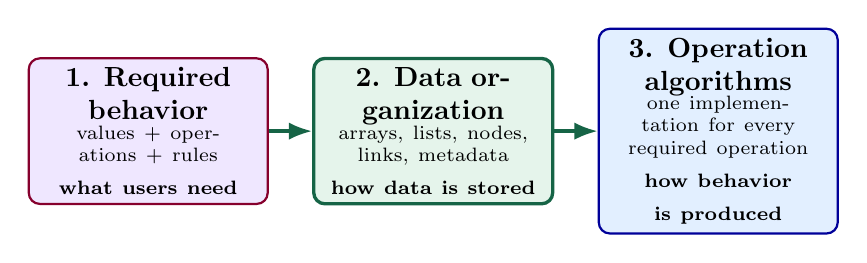
\begin{tikzpicture}[node distance=0.55cm]
      \node[adtbox,text width=2.8cm] (adt) {
        \textbf{1. Required behavior}\\[-0.1em]
        \scriptsize values + operations + rules\\
        \textbf{what users need}
      };
      \node[concept,text width=2.8cm,right=of adt] (representation) {
        \textbf{2. Data organization}\\[-0.1em]
        \scriptsize arrays, lists, nodes, links, metadata\\
        \textbf{how data is stored}
      };
      \node[application,text width=2.8cm,right=of representation] (algorithms) {
        \textbf{3. Operation algorithms}\\[-0.1em]
        \scriptsize one implementation for every required operation\\
        \textbf{how behavior is produced}
      };
      \draw[arrow] (adt) -- (representation);
      \draw[arrow] (representation) -- (algorithms);
    \end{tikzpicture}
  \end{center}

  \vspace{0.35em}
  \begin{center}
    \setlength{\tabcolsep}{4pt}
    \renewcommand{\arraystretch}{1.02}
    \begin{tabular}{L{0.17\textwidth}L{0.33\textwidth}L{0.39\textwidth}}
      \toprule
      \textbf{Design part} & \textbf{Question to answer} & \textbf{Python list example} \\
      \midrule
      Public contract & Which values, operations, results, and rules are visible? &
        Ordered mutable sequence: access, update, append, insert, and remove \\
      Data organization & How are elements and supporting state arranged? &
        Elements are maintained in index order by a built-in \texttt{list} object \\
      Operation implementation & Which algorithm realizes each operation and preserves the rules? &
        \texttt{items[i]}, \texttt{items[i] = x}, \texttt{append}, \texttt{insert}, and \texttt{pop} \\
      \bottomrule
    \end{tabular}
  \end{center}

  \vspace{0.10em}
  \centering
  \textbf{Design order:} specify required behavior $\rightarrow$ organize the data
  $\rightarrow$ implement and test every operation.
\end{frame}


\begin{frame}{Quiz: workload-driven structure selection}
\footnotesize
\begin{block}{Scenario}
A library system must frequently check whether a book ID is currently borrowed.
It occasionally adds a newly borrowed ID and removes a returned ID.
The display order of IDs is not important.
\end{block}
\quizblock{
Which structure is the most suitable initial choice, and why?
\begin{enumerate}
  \item Python \texttt{list}
  \item Python \texttt{tuple}
  \item Python \texttt{set}
  \item Python \texttt{dict}
\end{enumerate}}
\vspace{0.25em}
\begin{alertblock}{Reasoning prompt}
Base your choice on the required operations: membership test, insertion,
deletion, ordering, and uniqueness.
\end{alertblock}
\end{frame}

\begin{frame}{Quiz: data type or data structure?}
\small
\quizblock{Classify each item as mainly about \textbf{data type}, \textbf{data structure}, or \textbf{operation/workload requirement}.}
\vspace{0.3em}
\begin{enumerate}
  \item A value is an integer and supports arithmetic operations.
  \item Values are organized in a sequence so that the $i$-th element can be accessed.
  \item The program must frequently test whether an ID is present.
  \item A graph stores relationships among users in a social network.
  \item A Boolean value represents a true/false condition.
\end{enumerate}
\end{frame}

% =============================================================
\section{Abstract Data Types}
% =============================================================

\begin{frame}{Abstract Data Type (ADT)}
  \begin{columns}[T]
    \begin{column}{0.46\textwidth}
      \begin{block}{Definition}
        An ADT specifies a collection of data together with the operations and
        behavioral rules available to users.
      \end{block}

      \begin{exampleblock}{Focus}
        The ADT describes \textbf{what} can be done, not exactly \textbf{how}
        it is implemented.
      \end{exampleblock}
    \end{column}
    \begin{column}{0.50\textwidth}
      \begin{center}
        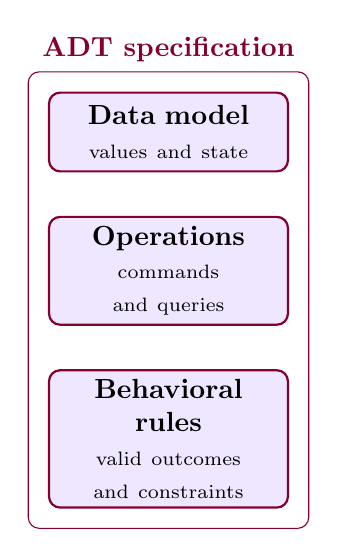
\begin{tikzpicture}[node distance=0.55cm]
          \node[adtbox] (data) {\textbf{Data model}\\\scriptsize values and state};
          \node[adtbox, below=of data] (ops) {\textbf{Operations}\\\scriptsize commands and queries};
          \node[adtbox, below=of ops] (rules) {\textbf{Behavioral rules}\\\scriptsize valid outcomes and constraints};
          \node[draw=purple!70!black, rounded corners, fit=(data)(ops)(rules), inner sep=0.25cm,
            label={[purple!70!black]above:\textbf{ADT specification}}] {};
        \end{tikzpicture}
      \end{center}
    \end{column}
  \end{columns}
\end{frame}

\begin{frame}{Example ADT: Set}
\footnotesize
\begin{columns}[T]
\begin{column}{0.45\textwidth}
\begin{block}{Data}
A \textbf{Set ADT} represents a collection of \textbf{unique elements}.
\end{block}

\begin{exampleblock}{Operations}
\begin{itemize}
  \item \texttt{add(x)}, \texttt{remove(x)}
  \item \texttt{contains(x)}
  \item \texttt{size()}, \texttt{is\_empty()}
  \item \texttt{union(S)}
  \item \texttt{intersection(S)}
  \item \texttt{difference(S)}
\end{itemize}
\end{exampleblock}
\end{column}

\begin{column}{0.52\textwidth}
\begin{center}
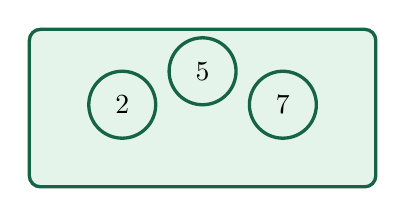
\begin{tikzpicture}[scale=0.85]
  \node[draw=ForestGreen,very thick,fill=SoftGreen,
    rounded corners,minimum width=4.4cm,minimum height=2cm] at (1.5,0.1) {};

  \node[draw=ForestGreen,very thick,fill=SoftGreen,
    circle,minimum size=0.85cm] at (0.3,0.15) {2};

  \node[draw=ForestGreen,very thick,fill=SoftGreen,
    circle,minimum size=0.85cm] at (1.5,0.65) {5};

  \node[draw=ForestGreen,very thick,fill=SoftGreen,
    circle,minimum size=0.85cm] at (2.7,0.15) {7};
\end{tikzpicture}

\vspace{-0.2em}
\[
S=\{2,5,7\}
\]
\end{center}

\begin{alertblock}{Rules}
\begin{itemize}
  \item No duplicate values.
  \item No index positions.
  \item Adding an existing element changes nothing.
\end{itemize}
\end{alertblock}
\end{column}
\end{columns}
\end{frame}

\begin{frame}{Set ADT: what vs. how}
\footnotesize

\begin{center}
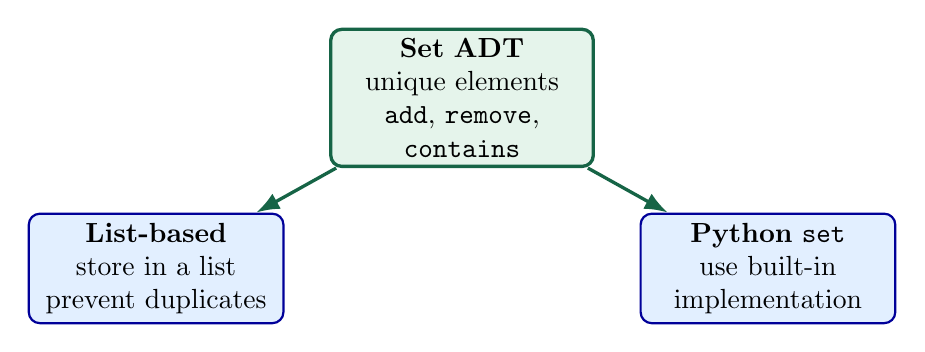
\begin{tikzpicture}[node distance=0.8cm]
  \node[concept, text width=3.1cm] (adt) {
    \textbf{Set ADT}\\
    unique elements\\
    \texttt{add}, \texttt{remove}, \texttt{contains}
  };

  \node[application, below left=of adt, text width=3.0cm] (list) {
    \textbf{List-based}\\
    store in a list\\
    prevent duplicates
  };

  \node[application, below right=of adt, text width=3.0cm] (pythonset) {
    \textbf{Python \texttt{set}}\\
    use built-in\\
    implementation
  };

  \draw[arrow] (adt) -- (list);
  \draw[arrow] (adt) -- (pythonset);
\end{tikzpicture}
\end{center}

\vspace{-0.4em}

\begin{columns}[T]
\begin{column}{0.48\textwidth}
\begin{block}{User knows}
\begin{itemize}
  \item Supported operations
  \item Duplicate rule
  \item Returned results
\end{itemize}
\end{block}
\end{column}

\begin{column}{0.48\textwidth}
\begin{alertblock}{User need not know}
\begin{itemize}
  \item Internal storage
  \item Membership checking
  \item Duplicate prevention
\end{itemize}
\end{alertblock}
\end{column}
\end{columns}

\vspace{-0.2em}

\[
S=\{2,5,7\},\quad \texttt{add(5)} \Rightarrow S=\{2,5,7\}
\]

\centering
\textbf{ADT specifies behavior; implementation decides how.}
\end{frame}


\begin{frame}{ADT versus data structure}
  \begin{center}
    \begin{tabular}{p{0.42\textwidth}p{0.42\textwidth}}
      \toprule
      \textbf{Abstract Data Type} & \textbf{Data Structure / Implementation} \\
      \midrule
      Describes required behavior & Describes concrete organization \\
      \addlinespace
      Focuses on operations and rules & Focuses on memory and algorithms \\
      \addlinespace
      Answers: ``What can the user do?'' & Answers: ``How is it built?'' \\
      \addlinespace
      Examples: Set, sequence, key--value map & Examples: array, linked list, hash table \\
      \bottomrule
    \end{tabular}
  \end{center}

  \vspace{0.55em}
  \begin{empheq}[box=\tcbhighmath]{equation*}
    \text{ADT = specification \qquad Data structure = realization}
  \end{empheq}
\end{frame}

\begin{frame}{Activity: unique course registrations}
  \small
  \begin{block}{Scenario}
    A registration program stores course codes. A course may appear only once,
    and the program must add, remove, and check registered courses.
  \end{block}
  \begin{columns}[T]
    \begin{column}{0.48\textwidth}
      \begin{exampleblock}{Questions}
        \begin{enumerate}
          \item What data should be stored?
          \item What is the type of one item?
          \item Which ADT describes the required behavior?
          \item How can a Python \texttt{list} implement it?
        \end{enumerate}
      \end{exampleblock}
    \end{column}
    \begin{column}{0.48\textwidth}
      \quizblock{
      Write a short design note that separates:
      \begin{enumerate}
        \item the ADT-level behavior;
        \item the concrete storage choice;
        \item the algorithm for avoiding duplicates.
      \end{enumerate}}
    \end{column}
  \end{columns}
\end{frame}


\begin{frame}{Quiz: ADT or implementation?}
\small
\quizblock{For each statement, decide whether it describes an \textbf{ADT specification} or a \textbf{concrete implementation}.}
\vspace{0.3em}
\begin{enumerate}
  \item A Set contains no duplicate elements.
  \item Elements are stored internally in a Python list.
  \item \texttt{contains(x)} returns whether \texttt{x} belongs to the collection.
  \item Membership is checked by scanning from left to right.
  \item A dictionary maps each key to an associated value.
\end{enumerate}
\vspace{0.35em}
\begin{alertblock}{Central distinction}
Ask whether the statement describes \textbf{what users can rely on} or
\textbf{how one implementation produces that behavior}.
\end{alertblock}
\end{frame}

\begin{frame}{Quiz: Set ADT behavior}
\small
\quizblock{Suppose a Set ADT currently contains $S=\{2,5,7\}$. Predict the result of each operation at the ADT level.}
\vspace{0.35em}
\begin{enumerate}
  \item \texttt{add(5)}
  \item \texttt{add(9)}
  \item \texttt{remove(2)}
  \item \texttt{contains(7)}
  \item \texttt{contains(4)}
\end{enumerate}
\vspace{0.35em}
\begin{exampleblock}{Discussion prompt}
Which of these predictions depend on the internal representation?
\end{exampleblock}
\end{frame}

% =============================================================
% WRAP-UP
% =============================================================
\begin{frame}{Connecting the four concepts}
  \begin{center}
    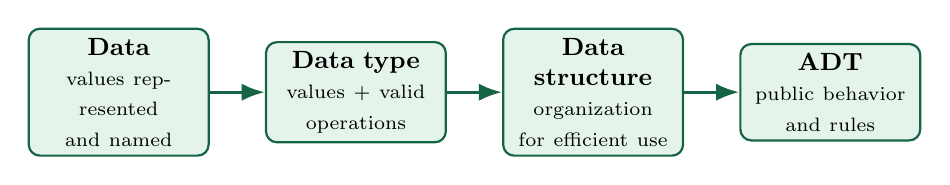
\begin{tikzpicture}[node distance=0.7cm]
      \node[stage] (variable) {\textbf{Data}\\\scriptsize values represented and named};
      \node[stage, right=of variable] (type) {\textbf{Data type}\\\scriptsize values + valid operations};
      \node[stage, right=of type] (structure) {\textbf{Data structure}\\\scriptsize organization for efficient use};
      \node[stage, right=of structure] (adt) {\textbf{ADT}\\\scriptsize public behavior and rules};
      \draw[arrow] (variable) -- (type);
      \draw[arrow] (type) -- (structure);
      \draw[arrow] (structure) -- (adt);
    \end{tikzpicture}
  \end{center}

  \vspace{0.7em}
  \begin{alertblock}{Central lesson}
    Good program design separates what users need from how data is stored and
    manipulated internally.
  \end{alertblock}
\end{frame}


\begin{frame}{Final review quiz}
\footnotesize
\quizblock{Match each concept on the left with the most appropriate description on the right.}
\vspace{0.3em}
\begin{columns}[T]
\begin{column}{0.43\textwidth}
\begin{block}{Concept}
\begin{enumerate}
  \item Data
  \item Data type
  \item Data structure
  \item ADT
  \item Implementation
\end{enumerate}
\end{block}
\end{column}
\begin{column}{0.52\textwidth}
\begin{exampleblock}{Description}
\begin{enumerate}
  \item[A.] A concrete way to store data and realize operations.
  \item[B.] Facts or observations represented in a program.
  \item[C.] A specification of public behavior and rules.
  \item[D.] A set of values and valid operations.
  \item[E.] An organization of many values for effective use.
\end{enumerate}
\end{exampleblock}
\end{column}
\end{columns}
\end{frame}

\begin{frame}{Exit ticket}
  \begin{enumerate}
    \item In \texttt{scores = [8, 7, 9]}, identify the data, variable name, and object type.
    \item Why can the same Set ADT be implemented with either a Python list or a built-in set?
    \item Classify each as an ADT or a concrete implementation: Set ADT, Python list, Python set, linked list.
  \end{enumerate}

  \vspace{0.7em}
  \begin{exampleblock}{Prepare for the next topic}
    Next, object-oriented programming will package related state, operations,
    and rules inside classes that can implement reusable ADTs.
  \end{exampleblock}
\end{frame}

\begin{frame}{Key takeaway}
  \fcolorbox{black}{yellow!20}{%
    \begin{minipage}{\dimexpr\linewidth-2\fboxsep-2\fboxrule}
      \textbf{Programs represent data as values accessed through variable names.
      Types define valid values and operations.
      Data structures organize collections of values. ADTs define the public
      behavior independently of implementation. These distinctions allow us to
      design software that is clearer, safer, and easier to optimize.}
    \end{minipage}%
  }

  \vspace{1.0em}
  \centering
  \Large Next: object-oriented programming.
\end{frame}

\begin{frame}{}

{\Huge\color{ForestGreen}
\centering{\bfseries Any Questions?}
}

\end{frame}

\end{document}
